\documentclass[12pt]{beamer}

\usetheme{Oxygen}
\usepackage{thumbpdf}
\usepackage{wasysym}
% \usepackage{ucs}
\usepackage[utf8]{inputenc}
\usepackage{pgf,pgfarrows,pgfnodes,pgfautomata,pgfheaps,pgfshade}
\usepackage{verbatim}

\pdfinfo
{
  /Title       (Ingeniería de Software)
  /Creator     (TeX)
  /Author      (Sebastián Salazar Molina)
}


\title{Ingeniería de Software}
\subtitle{Metodologías de Desarrollo}
\author{Sebastián Salazar Molina.}
\institute[INF - UTEM] { Unidad de Informática - Universidad Tecnológica Metropolitana }
\date{06 de Abril de 2015}

\begin{document}

\frame{\titlepage}

\section*{}
\begin{frame}
  \frametitle{Contenidos}
  \tableofcontents[section=1,hidesubsections]
\end{frame}

\AtBeginSection[]
{
  \frame<handout:0>
  {
    \frametitle{Contenidos}
    \tableofcontents[currentsection,hideallsubsections]
  }
}

\AtBeginSubsection[]
{
  \frame<handout:0>
  {
    \frametitle{Contenidos}
    \tableofcontents[sectionstyle=show/hide,subsectionstyle=show/shaded/hide]
  }
}

\newcommand<>{\highlighton}[1]{%
  \alt#2{\structure{#1}}{{#1}}
}

\newcommand{\icon}[1]{\pgfimage[height=1em]{#1}}



%%%%%%%%%%%%%%%%%%%%%%%%%%%%%%%%%%%%%%%%%
%%%%%%%%%% Content starts here %%%%%%%%%%
%%%%%%%%%%%%%%%%%%%%%%%%%%%%%%%%%%%%%%%%%



% Metodologías
\section{Introducción}
\subsection{Introducción.}

\begin{frame}
 \begin{quote}
  Mide lo que sea medible y haz medible lo que no lo sea.
 \newline
 \raggedleft{-- Galileo Galilei.}
 \end{quote}
\end{frame}


\subsection{Problema del Software}

\begin{frame}
\frametitle{Problema}
  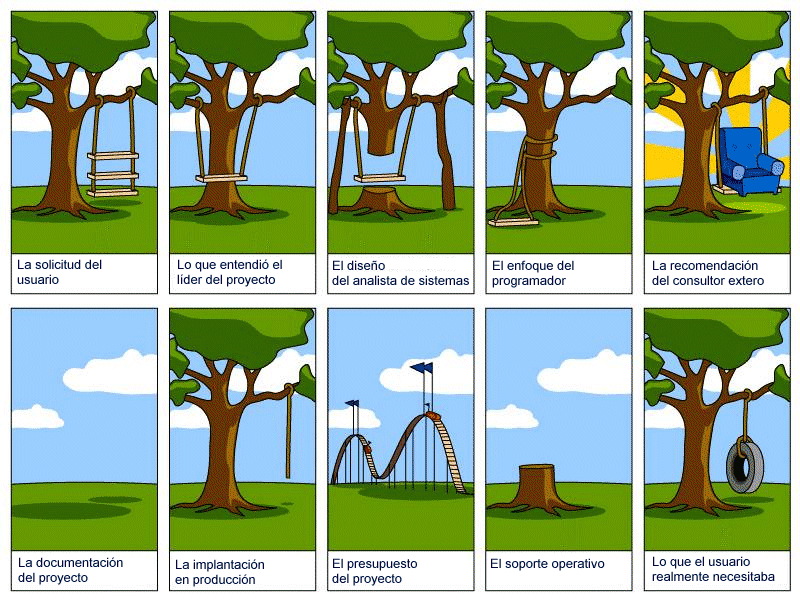
\includegraphics[scale=0.30]{img/sin-metodologias.png}
\end{frame}




\begin{frame}
\frametitle{Solución}
  \begin{itemize}
   \item<1-> Entender el problema.
   \item<2-> Buscar la mejor alternativa.
   \item<3-> Estimar el esfuerzo necesario.
   \item<4-> Generar un plan de trabajo.
   \item<5-> Usar \alert{metodologías}.
  \end{itemize}
\end{frame}


\begin{frame}
 \frametitle{Método Científico}
  La definición típica del método científico, fue dada por Francis Bacon, y es la siguiente:
  \begin{itemize}
   \item<2-> \alert{Observación} Observar es aplicar atentamente los sentidos a un objeto o a un fenómeno, para estudiarlos tal como se presentan en realidad, puede ser ocasional o causalmente.
   \item<3-> \alert{Inducción} La acción y efecto de extraer, a partir de determinadas observaciones o experiencias particulares, el principio particular de cada una de ellas.
   \item<4-> \alert{Hipótesis} Planteamiento mediante la observación siguiendo las normas establecidas por el método científico.
   \item<5-> Probar la hipótesis por \alert{experimentación}.
   \item<6-> \alert{Demostración} o \alert{refutación} (antítesis) de la hipótesis.
   \item<7-> Tesis o teoría científica (\alert{conclusiones}).
  \end{itemize}
\end{frame}


\subsection{Metodología de Desarrollo de Software}
\begin{frame}
 \frametitle{Metodología de Desarrollo de Software}
 Una Metodología de desarrollo de software es un marco de trabajo usado para estructurar, planificar y controlar el proceso de desarrollo en sistemas de información.
\end{frame}


\begin{frame}
 \frametitle{Enfoques}
 Existen muchas metodologías de desarrollo, cada uno tiene un enfoque diferente.
 \newline
 \begin{itemize}
  \item<2-> Desarrollo en Cascada.
  \item<3-> Prototipado.
  \item<4-> Desarrollo iterativo y creciente
  \item<5-> Desarrollo en Espiral
  \item<6-> ...
  \item<7-> Desarrollo Ágil
 \end{itemize}

\end{frame}


\begin{frame}
 \frametitle{Desarrollo en Cascada}
 \begin{itemize}
  \item Análisis de requisitos.
  \item Diseño del Sistema.
  \item Diseño del Programa.
  \item Codificación.
  \item Pruebas.
  \item Implantación.
  \item Mantenimiento.
 \end{itemize}
\end{frame}



\begin{frame}
 \frametitle{Prototipado}
 \begin{itemize}
  \item Plan rápido
  \item Modelado, diseño rápido
  \item Construcción del Prototipo
  \item Desarrollo, entrega y retroalimentación
  \item Comunicación 
 \end{itemize}
\end{frame}


\begin{frame}
 \frametitle{Desarrollo iterativo y creciente}
 \begin{itemize}
  \item Etapa de inicialización
  \item Etapa de iteración
  \item Lista de control de proyecto
 \end{itemize}
\end{frame}


\begin{frame}
 \frametitle{Desarrollo en Espiral}
 \begin{itemize}
  \item Determinar Objetivos.
  \item Análisis del riesgo.
  \item Planificación.
  \item Desarrollar y probar. 
 \end{itemize}
\end{frame}

\subsection{Desarrollo Ágil}

\begin{frame}
 \frametitle{Desarrollo Ágil}
 El desarrollo ágil de software son métodos basados en el desarrollo iterativo e incremental, donde los requerimientos y soluciones \alert{evolucionan}.
 \newline
 Los riesgos se minimizan, desarrollando unidades de software de funcionalidad acotada en lapsos de tiempos breves (usualmente ciclos de 1 a 4 semanas), que se denominan \alert{iteraciones}.
 \newline
 En cada iteración, se deben realizar las siguientes actividades: Planificación, Análisis de requerimientos, Diseño, Codificación, Revisión y Documentación. Al final de cada iteración el equipo vuelve a evaluar las prioridades del proyecto.
\end{frame}


\begin{frame}
 \frametitle{Metodologías Ágiles}
 Existen una gran variedad de metodologías Ágiles, entre ellas destacan:
 \begin{itemize}
  \item<2-> Programación Extrema.
  \item<3-> Scrum.
  \item<4-> Kanban.
  \item<5-> Largo etc...
 \end{itemize}
\end{frame}


\begin{frame}
 \begin{quote}
  La mayoría de ustedes están familiarizados con las virtudes del programador. Son tres, por supuesto: pereza, impaciencia y orgullo desmedido
 \newline
 \raggedleft{-- Larry Wall.}
 \end{quote}
\end{frame}


\subsection{Virtudes}

\begin{frame}
 \frametitle{Virtudes del programador}
 \begin{itemize}
  \item<2-> \alert{Pereza}. Es la cualidad que te hace realizar un gran esfuerzo para reducir el total del gasto energético (hacerlo bien a la primera). Te hace escribir programas que ahorren trabajo y que otras personas encontrarán útil, documentar lo que escribes para no tener que responder muchas preguntas sobre él.
  \item<3-> \alert{Impaciencia}. Se puede resumir como la ira que se siente cuando el ordenador se está volviendo lento. Esto te hace escribir programas que no solo reaccionan a tus necesidades, sino que se anticipen a ellas. O al menos lo pretendan.
  \item<4-> \alert{Orgullo Desmedido}. Es la cualidad que te hace escribir (y mantener) programas de los cuales otras personas no puedan decir cosas malas. 
  \end{itemize}
\end{frame}

\section{Desarrollo Ágil}


\subsection{Problemas comunes}
\begin{frame}
 \frametitle{Problemas comunes}
 Existen problemas típicos, asociados al desarrollo de software (Requerimientos mal definidos, malas estimaciones, etc...).
 \newline
 Las crisis no se arreglan gritando o presionando más, sino que requieren un trabajo \alert{ordenado} y que las partes reconozcan su responsabilidad. Eso realmente es lo más importante y difícil para solventar la crisis, reconocer que hay un problema y que se ha sido parte de él.
\end{frame}

\begin{frame}
 \frametitle{Desarrollo Ágil}
 El desarrollo ágil, es una respuesta \alert{metodológica} a los problemas actuales del desarrollo de Software. Su principal objetivo es organizar mejor su proyecto y obtener un mejor resultado del software entregado a su cliente.
\end{frame}


\begin{frame}
 \frametitle{Desarrollo Ágil}
 El desarrollo ágil de software son métodos basados en el desarrollo iterativo e incremental, donde los requerimientos y soluciones \alert{evolucionan}.
 \newline
 Los riesgos se minimizan, desarrollando unidades de software de funcionalidad acotada en lapsos de tiempos breves (usualmente ciclos de 1 a 4 semanas), que se denominan \alert{iteraciones}.
 \newline
 En cada iteración, se deben realizar las siguientes actividades: Planificación, Análisis de requerimientos, Diseño, Codificación, Revisión y Documentación. Al final de cada iteración el equipo vuelve a evaluar las prioridades del proyecto.
\end{frame}

\subsection{Diferencias con las metodologías tradicionales}
\begin{frame}
 \frametitle{Base}
 Las Metodologías tradicionales se basan en \alert{estándares} que han sido ampliamente aceptadas por la industria. 
 \pause
 Las Metodologías ágiles se basan en la heurística, que proviene de la práctica de producción de código.
\end{frame}


\begin{frame}
 \frametitle{Heurística}
 Según la rae, la Heurística se define como:
 \newline
  (Del gr. εὑρίσκειν, hallar, inventar, y ‒tico).
  \begin{itemize}
   \item 1. adj. Perteneciente o relativo a la heurística.
   \item 2. f. Técnica de la indagación y del descubrimiento.
   \item 3. f. Busca o investigación de documentos o fuentes históricas.
   \item 4. f. En algunas ciencias, manera de buscar la solución de un problema mediante métodos no rigurosos, como por tanteo, reglas empíricas, etc.
  \end{itemize}

  \href{http://lema.rae.es/drae/?val=heurística}{Fuente: RAE}
\end{frame}


\begin{frame}
 \frametitle{Cambios}
 Las metodologías tradicionales tiene una alta resistencia a los cambios, mientras que las metodologías ágiles están preparados abordar el cambio y evolucionar con él.
\end{frame}


\begin{frame}
 \frametitle{Procesos de desarrollo}
 La forma tradicional de trabajo tiene un conjunto elevado de normas y políticas, las metodologías ágiles, tienen procesos menos controlados y pocas restricciones.
\end{frame}

\begin{frame}
 \frametitle{Situación Contractual}
 Las metodologías tradicionales, existe un contrato formal y definido, en el enfoque ágil, el contrato es flexible.
\end{frame}


\begin{frame}
 \frametitle{Cliente}
 La forma tradicional de trabajar con el cliente, es basado en reuniones. El enfoque ágil, el cliente debe ser parte del equipo de desarrollo.
\end{frame}

\begin{frame}
 \frametitle{Grupos de trabajo}
 La idea tradicional es usar mucha gente en los equipos. Las metodologías ágiles, es utilizar grupos pequeños fuertemente motivados.
\end{frame}


\begin{frame}
 \frametitle{Roles y Arquitectura}
 El enfoque tradicional tiene una fuerte jerarquía, con una arquitectura rígida. La idea ágil, es usar pocos roles y una arquitectura flexible, el énfasis está en los resultados.
\end{frame}


\subsection{Filosofía}

\begin{frame}
 \frametitle{Manifiesto Ágil}
 El 17 de febrero de 2001, se reunieron en Snowbird, Utah, las siguientes personas:  Kent Beck, Mike Beedle, Arie van Bennekum, Alistair Cockburn, Ward Cunningham, Martin Fowler, James Grenning, Jim Highsmith, Andrew Hunt, Ron Jeffries, Jon Kern, Brian Marick, Robert C. Martin, Steve Mellor, Ken Schwaber, Jeff Sutherland y Dave Thomas para tratar sobre técnicas y procesos para desarrollar software. En la reunión se acuñó el término ``Métodos Ágiles'' para definir a los métodos que estaban surgiendo como alternativa a las metodologías formales (rígidas y normativas).
\end{frame}


\begin{frame}
 \frametitle{Valores del Manifiesto Ágil}
 Se valora a: 
 \begin{itemize}
  \item<2-> Los individuos y su interacción, por encima de los procesos y las herramientas.
  \item<3-> El software que funciona, por encima de la documentación exhaustiva.
  \item<4-> La colaboración con el cliente, por encima de la negociación contractual.
  \item<5-> La respuesta al cambio, por encima del seguimiento de un plan.
 \end{itemize}
\end{frame}



\begin{frame}
 \frametitle{Principios del Manifiesto Ágil}
 \begin{itemize}
  \item<2-> Nuestra principal prioridad es satisfacer al cliente a través de la entrega temprana y continua de software de valor.
  \item<3-> Son bienvenidos los requisitos cambiantes, incluso si llegan tarde al desarrollo. Los procesos ágiles se doblegan al cambio como ventaja competitiva para el cliente.
  \item<4-> Entregar con frecuencia software que funcione, en periodos de un par de semanas hasta un par de meses, con preferencia en los periodos breves.
  \item<5-> Las personas del negocio y los desarrolladores deben trabajar juntos de forma cotidiana a través del proyecto.
\end{itemize}
\end{frame}  
  
\begin{frame}
 \frametitle{Principios del Manifiesto Ágil}
 \begin{itemize}
  \item<2-> Construcción de proyectos en torno a individuos motivados, dándoles la oportunidad y el respaldo que necesitan y procurándoles confianza para que realicen la tarea.
  \item<3-> La forma más eficiente y efectiva de comunicar información de ida y vuelta dentro de un equipo de desarrollo es mediante la conversación cara a cara.
  \item<4-> El software que funciona es la principal medida del progreso.
  \item<5-> Los procesos ágiles promueven el desarrollo sostenido. Los patrocinadores, desarrolladores y usuarios deben mantener un ritmo constante de forma indefinida.
  
 \end{itemize}
\end{frame}


\begin{frame}
 \frametitle{Principios del Manifiesto Ágil}
 \begin{itemize}
  \item<2-> La atención continua a la excelencia técnica enaltece la agilidad.
  \item<3-> La simplicidad como arte de maximizar la cantidad de trabajo que no se hace, es esencial.
  \item<4-> Las mejores arquitecturas, requisitos y diseños emergen de equipos que se auto-organizan.
  \item<5-> En intervalos regulares, el equipo reflexiona sobre la forma de ser más efectivo y ajusta su conducta en consecuencia.
 \end{itemize}
\end{frame}


% Scrum
\section{Scrum}
\subsection{Introducción.}

\begin{frame}
 \begin{quote}
  No soy el único de mi equipo, pero en mi equipo soy único.
 \newline
 \raggedleft{-- Gregory House.}
 \end{quote}
\end{frame}


\subsection{Rugby}


\begin{frame}
 \frametitle{Origen}
 La melé o el ``scrum'', una de las formaciones más reconocibles del rugby, es una puja frente a frente, de un grupo de cada equipo, que se presentan agachados y agarrados, para comenzar a empujar con el fin de obtener el balón que ha sido lanzado en medio de ellos y sin tocarlo con la mano. El grupo que haya obtenido el balón, debe sacarlo sin tocarlo con la mano por detrás de la formación, donde lo tomará un jugador (usualmente, pero no siempre, el "medio melé" o "medio scrum") y continuará el juego.
\end{frame}



\begin{frame}
\frametitle{Rugby}
  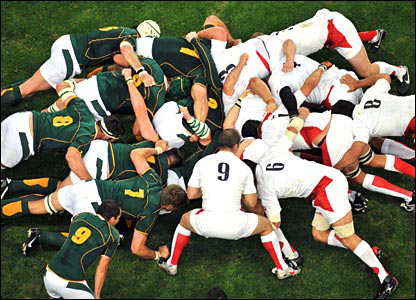
\includegraphics[scale=0.5]{img/scrum_rugby.png}
\end{frame}
\subsection{Scrum}

\begin{frame}
 \frametitle{Introducción}
 Scrum es un modelo de ``referencia'' que define un conjunto de \alert{prácticas} y \alert{roles}, y que puede tomarse como punto de partida para definir el proceso de desarrollo que se ejecutará durante un proyecto. 
 \newline
 Scrum permite la creación de equipos autoorganizados impulsando la co-localización de todos los miembros del equipo, y la \alert{comunicación} entre todos quienes estén \alert{involucrados} en el proyecto.
 \newline
 Un principio clave de Scrum es el reconocimiento de que durante un proyecto las necesidades y las prioridades pueden \alert{cambiar}. Lo bueno de Scrum, es que es muy fácil de aprender, y requiere muy poco esfuerzo para comenzarse a utilizar.
\end{frame}

\begin{frame}
 \frametitle{Roles}
 Las interacciones están definidas por los roles. En Scrum existen dos tipos de roles:
 \begin{itemize}
  \item<2-> Roles Principales
  \item<3-> Roles Auxiliares
 \end{itemize}
\end{frame}


\begin{frame}
 \frametitle{Roles Principales}
 
 \begin{itemize}
  \item<2-> El \alert{Product Owner} representa la voz del cliente. Se asegura de que el equipo Scrum trabaja de forma adecuada desde la perspectiva del negocio. El Product Owner escribe historias de usuario, las prioriza, y las coloca en el Product Backlog.
  \item<3-> El \alert{ScrumMaster}, cuyo trabajo primario es eliminar los obstáculos que impiden que el equipo alcance el objetivo del sprint. El ScrumMaster es el que hace que las reglas se cumplan.
  \item<4-> El \alert{equipo} tiene la responsabilidad de entregar el producto. Usualmente lo conforman de 3 a 9 personas con las habilidades transversales necesarias para realizar el trabajo (análisis, diseño, desarrollo, pruebas, documentación, etc). 
 \end{itemize}
\end{frame}


\begin{frame}
 \frametitle{Roles Secundarios}
 \begin{itemize}
  \item<2-> \alert{Stakeholders} Son quienes están involucrados en el proyecto y para quienes su construcción significa un beneficio. Durante un sprint sólo tienen voz.
  \item<3-> \alert{Managers} Son los administradores, la gente que establece el ambiente para el desarrollo del producto. 
 \end{itemize}

\end{frame}


\begin{frame}
 \frametitle{Sprint}
 El Sprint es el período en el que se trabaja. La duración se debe definir en base a la experiencia, aunque puede haber cierta flexibilidad en este punto. Al finalizar se debe cerrar el Sprint, con un producto funcional, con los objetivos y prioridades replanteados.
\end{frame}


\begin{frame}
 \frametitle{Reuniones}
 La comunicación es algo imprescindible y para lograrlo es necesario tener reuniones, en Scrum se definen algunas reunión:
 \begin{itemize}
  \item<2-> Daily Scrum. Son reuniones fijas, de 15 minutos, cada miembro debe responder: 
  1) ¿Qué has hecho desde ayer? 
  2) ¿Qué es lo que estás planeando hacer hoy? 
  3) ¿Has tenido algún problema que te haya impedido alcanzar tu objetivo?
  \item<3-> Scrum de Scrum. Son reuniones posteriores al Daily Scrum, y están orientadas a planificar mejor el trabajo, se usa cuando trabajan varios equipos.
 \end{itemize}
\end{frame}  

\begin{frame}
 \frametitle{Reuniones}
 \begin{itemize}
  \item<2-> Sprint Planning Meeting. Reunión de inicio y Planificación, tiene un límite de 8 horas.
  \item<3-> Sprint Review Meeting. Reunión Posterior al Sprint, para presentar y revisar el trabajo, máximo de 4 horas.
  \item<4-> Sprint Retrospective. Mejora Continua, máximo de 4 horas.
 \end{itemize}
\end{frame}


\begin{frame}
 \frametitle{Documentos}
 Scrum, define 1 Gráfico y 2 Documentos importantes:
 \begin{itemize}
  \item<2-> El product backlog.
  \item<3-> El sprint backlog.
  \item<4-> La burn down chart.
 \end{itemize}
\end{frame}


\begin{frame}
 \frametitle{Product Backlog}
 El product backlog es la lista de requerimientos del producto. El Product Owner es responsable Product Backlog. El Product Backlog nunca se acaba, y es usado para la planificación. Se desarrolla con el producto y evoluciona con él. Es dinámico; maneja constantemente los cambios para identificar que necesita el producto para ser: apropiado, competitivo, y útil. Mientras exista un producto, el Product Backlog también existe. 
\end{frame}


\begin{frame}
 \frametitle{Product Backlog}
 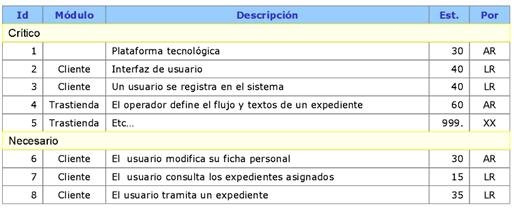
\includegraphics[scale=0.5]{img/product_backlog.png}
\end{frame}



\begin{frame}
 \frametitle{Sprint Backlog}
 El Sprint Backlog define las tareas a desarrollar en el Sprint, en un  incremento potencialmente funcional del producto. El equipo crea una lista inicial de estas tareas en la segunda parte del Sprint planning meeting Las tareas deben ser divididas de modo que cada una demore entre 4 a 16 horas finalizarlas. Las tareas de largo mayor de 16 horas se consideran secundarias, ya que todavía no se han definido apropiadamente. Solamente el equipo puede cambiar el Sprint Backlog. El Sprint Backlog es un cuadro altamente visible, es lo que debe conseguir durante una iteración del Sprint. 
\end{frame}


\begin{frame}
 \frametitle{Sprint Backlog}
 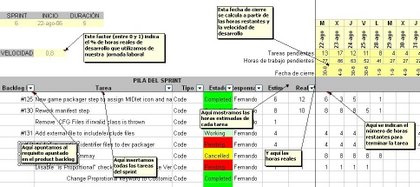
\includegraphics[scale=0.5]{img/sprint_backlog.png}
\end{frame}


\begin{frame}
 \frametitle{Burn down chart}
 El burn down chart demuestra la cantidad de trabajo restante a través de tiempo. La carta burndown es una manera excelente de visualizar la correlación entre la cantidad de trabajo restante en cualquier punto y el progreso de los equipos de proyecto en la reducción de este trabajo. La intersección de una línea de la tendencia para el trabajo restante y el eje horizontal indica el punto más probable en el que terminen las actividades. El burn down chart es el contraste entre la realidad (trabajo hecho y cuán rápidamente se está haciendo) y la planificación (lo esperado).
\end{frame}


\begin{frame}
 \frametitle{Burn down chart}
 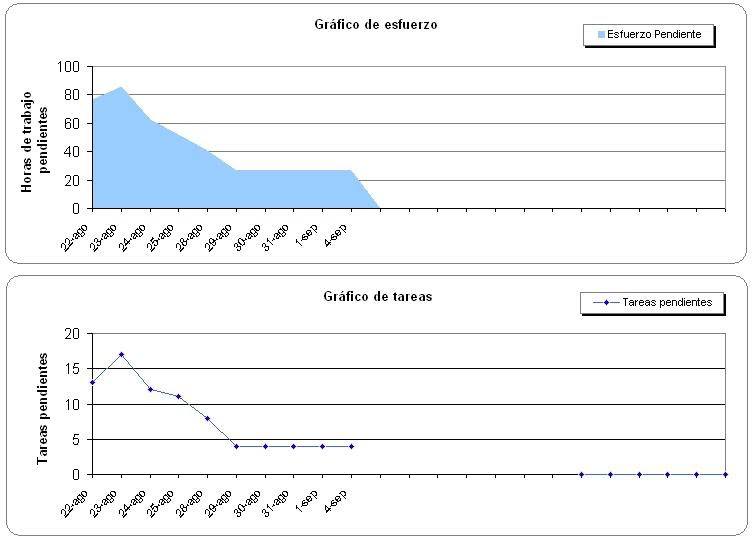
\includegraphics[scale=0.25]{img/bdc.png}
\end{frame}

\begin{frame}
 \frametitle{Ciclo de Trabajo}
 \begin{itemize}
  \item<2-> Toma de requerimientos. Se genera las historias de usuario.
  \item<3-> Se priorizan las historias.
  \item<4-> Se toma un conjunto de historias, que dan paso a un sprint.
  \item<5-> Al finalizar el sprint, se le hace entrega del producto al cliente.
 \end{itemize}

\end{frame}


\begin{frame}
\frametitle{Esquema}
  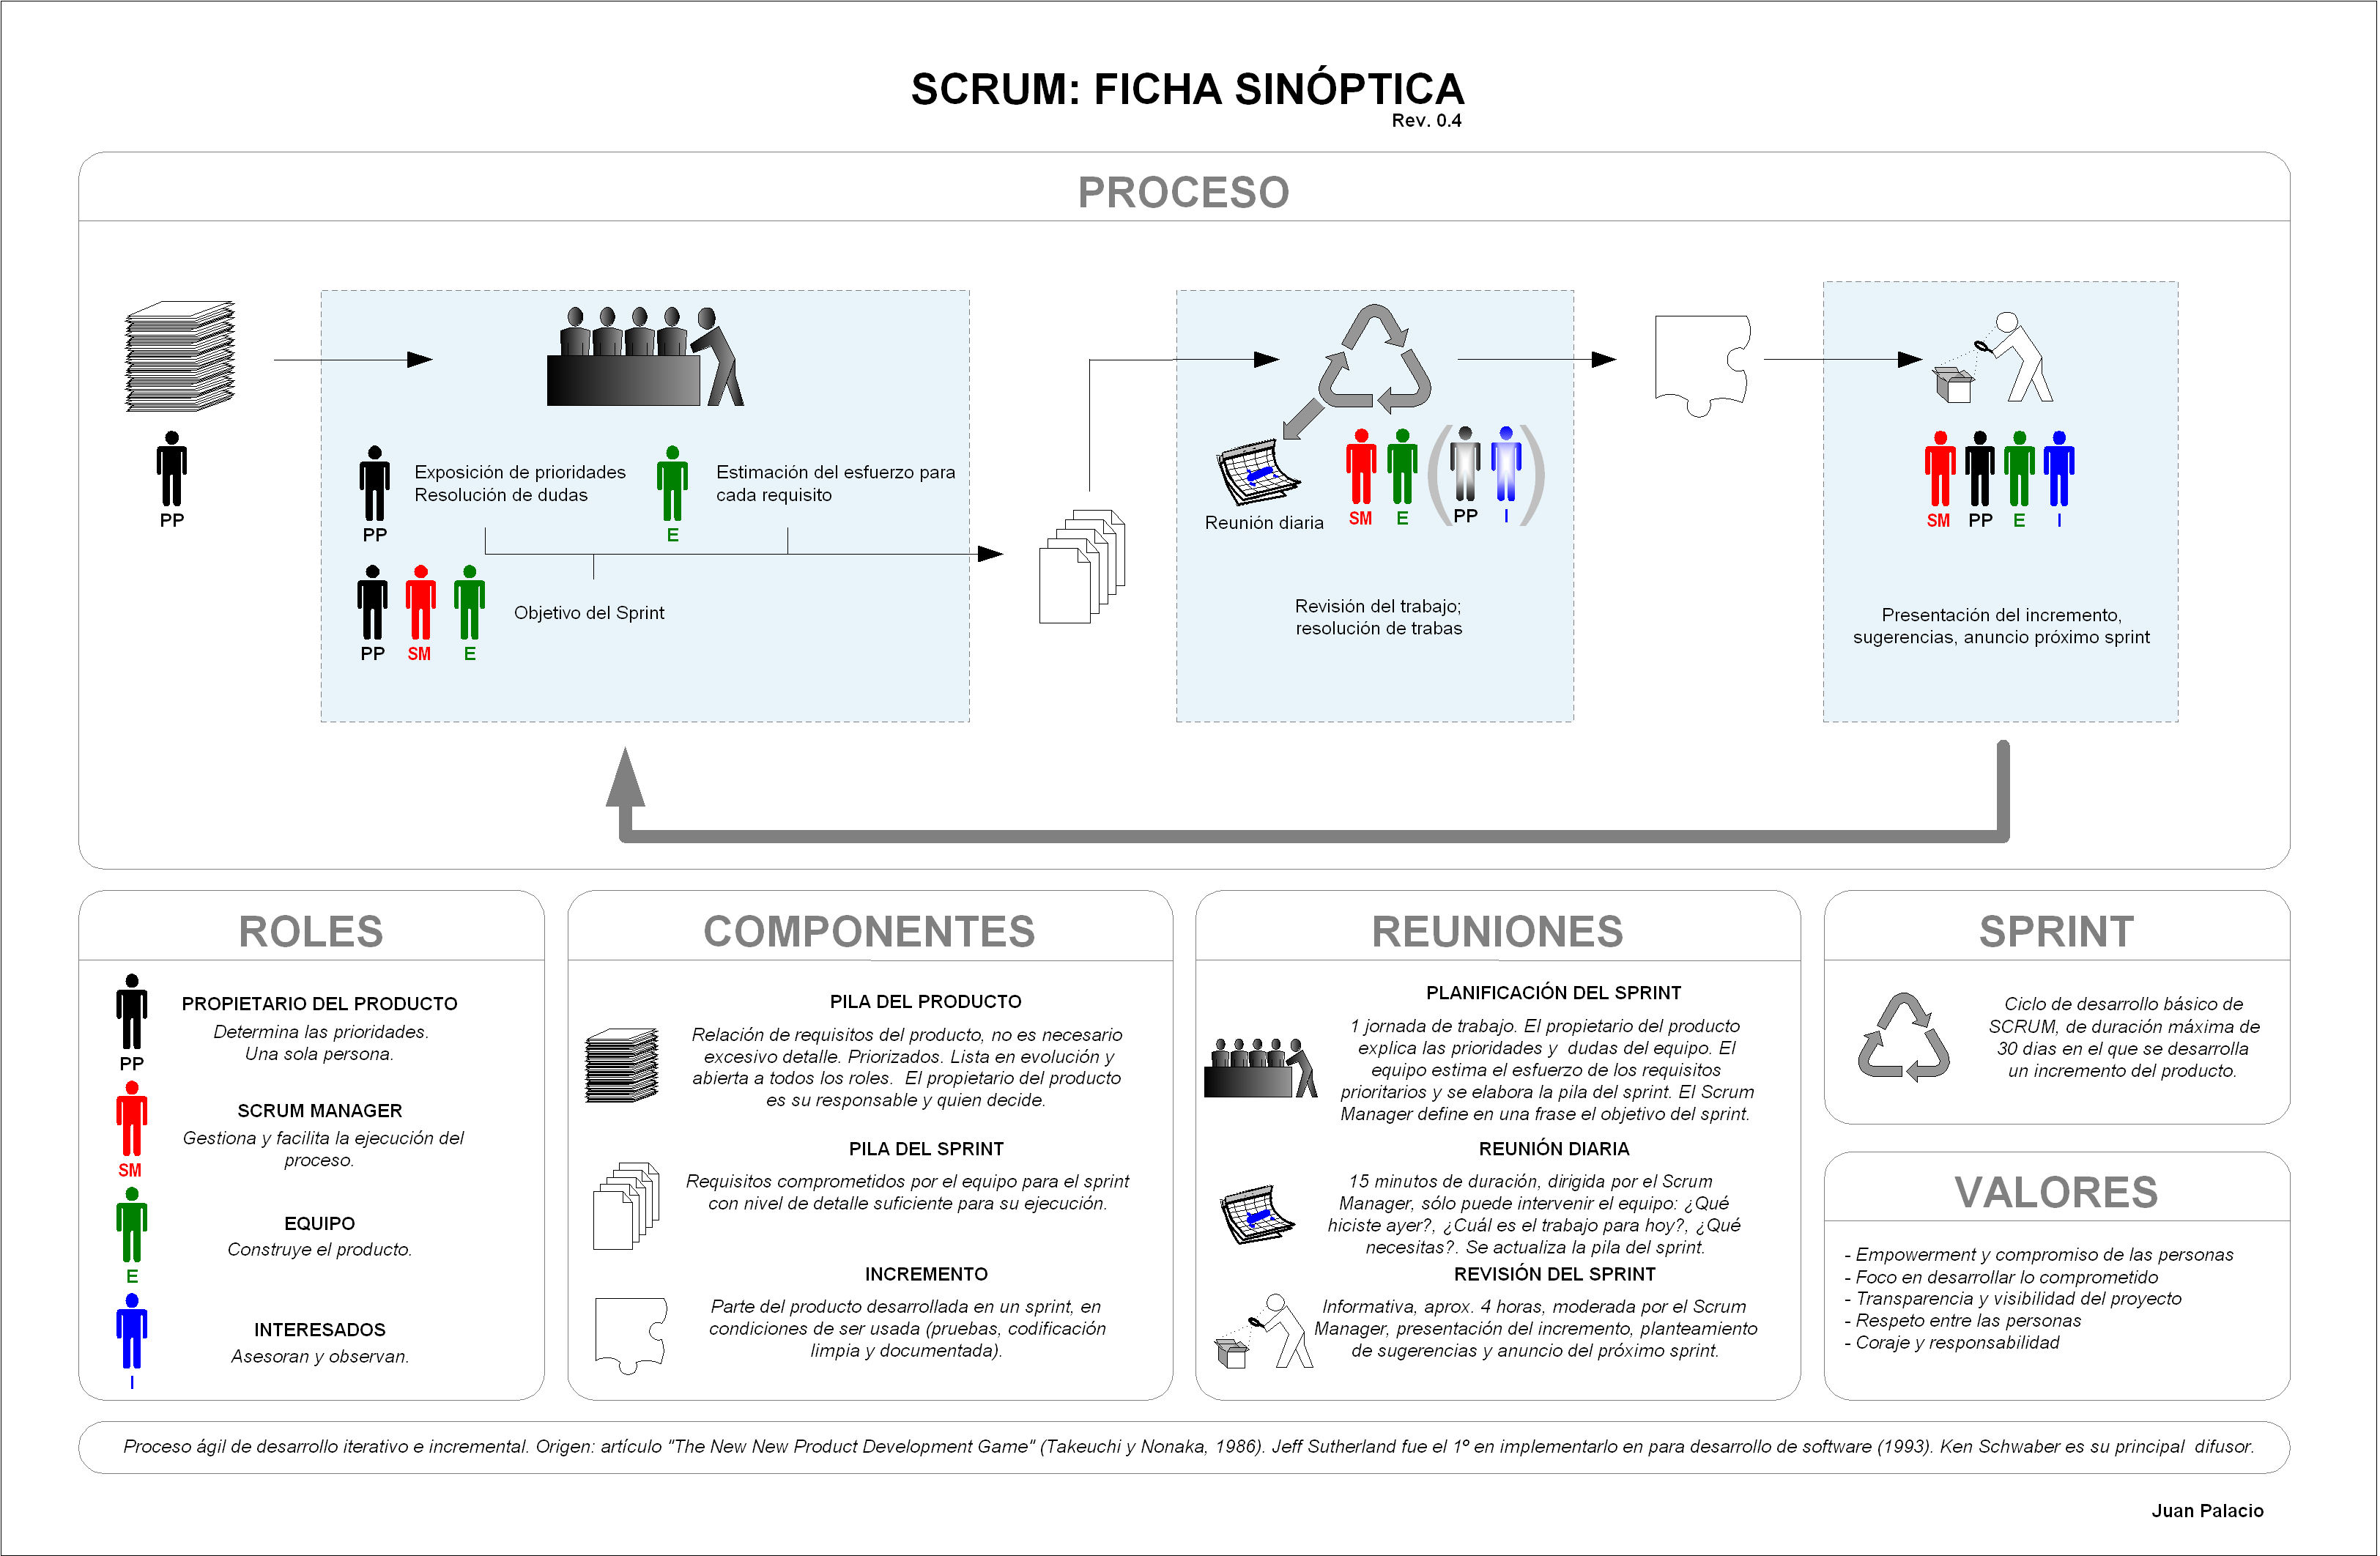
\includegraphics[scale=0.38]{img/Ficha_scrum.png}
\end{frame}



\frame{
  \vspace{2cm}
  {\huge ¿ Preguntas ?}

  \vspace{3cm}
  \begin{flushright}
    Sebastián Salazar Molina

    \structure{\footnotesize{sebasalazar@gmail.com}}
  \end{flushright}
}

\end{document}
